\chapter{Neural Networks} 


\label{Chapter2}

Neural networks, also known as \ac{ANN} are machine learning algorithms that form the basis of deep learning. They inherit name and structure from neurons in the brain. Biological neurons transmit signals to one another through complex networks. This interconnected networking is realized though various combinations of neurons forming an \ac{ANN}. Sets of artificial neurons are stacked on top of each other to form a layer. A typical neural network consists of many such layers that are connected to each other. The first layer is called input layer, the final layer is termed output layer and the layers in-between are called hidden layers. A neural network with three hidden layers is depicted in Fig~\ref{fig:nn}. The transmission of data across the nodes or artificial neurons happens through the connections. Each and every node has a specific weight and threshold associated. The output from a node is passed through the connection only if the value is above the threshold. Neural network approaches are data-driven. Their performance improves as they learn through training on a dataset. 

\begin{figure}
	\centering
\begin{neuralnetwork}[height=5]
	\newcommand{\x}[2]{$x_#2$}
	\newcommand{\y}[2]{$\hat{y}_#2$}
	\newcommand{\hfirst}[2]{\small $h^{(1)}_#2$}
	\newcommand{\hsecond}[2]{\small $h^{(2)}_#2$}
	\inputlayer[count=4, bias=true, title=Input\\layer, text=\x]
	\hiddenlayer[count=5, bias=false, title=Hidden\\layer 1, text=\hfirst] \linklayers
	\hiddenlayer[count=4, bias=false, title=Hidden\\layer 2, text=\hsecond] \linklayers
	\hiddenlayer[count=3, bias=false, title=Hidden\\layer 3, text=\hsecond] \linklayers
	\outputlayer[count=2, title=Output\\layer, text=\y] \linklayers
\end{neuralnetwork}
\caption{Depiction of a neural network with an input layer, three hidden layers and an output layer}\label{fig:nn}
\end{figure}


To further understand the working of a neural network, we can imagine each node to be solving the problem of linear regression. For example consider a node with four inputs ($x_i, i=1,2,\dots4$), four weights ($w_i, i=1,2,\dots4$) and a bias:

\begin{equation}
\sum_{i=1}^{m} w_{i} x_{i}+\text { bias }=w_{1} x_{1}+w_{2} x_{2}+w_{3} x_{3}+w_{4} x_{4}+\text { bias }
\end{equation}

The output of the node is the above summation after going through an activation function $g$:
\begin{equation}
\text { output }=g(x)=\left\{\begin{array}{l}
1 \text { if } \sum w_{1} x_{1}+b \geq 0 \\
0 \text { if } \sum w_{1} x_{1}+b<0
\end{array}\right.
\end{equation}
In the above example, the given activation function of this node propagates the value $1$ only when the weighted sum of it's inputs is non-negative. When the condition of an activation function are met, the output of this node becomes an input to the node to which it's connected. Due to the process of forwarding values through a network, an \ac{ANN} is also called feed-forward network. Complex networks with multiple layers of these nodes are used in practical tasks. An important category of machine learning task is supervised learning. It involves training a neural network on labeled datasets. The goal of training a neural network is to minimize a cost function that enforces the closeness of predicted and real output labels. During the training the network reorganizes it's weights based on the loss function. This process of updating weights is called optimization. Each update is aimed at reaching a minimum of the loss function. A popular optimization method is gradient descent. It guides the model in the direction of reducing errors to reach an optima. The development of back-propagation (\cite{rumelhart1986learning}) has been instrumental in successful implementation of optimization algorithms for neural networks. A machine learning algorithm is typically specified by a cost function, an optimization procedure and a model. Even neural network design is based on these principles. One can find a co-relation between the iterative reconstruction algorithms based on gradient-based optimization and neural network training with gradient descent. It is to be noted that the non-linearity in the activation functions causes moss functions to become non-convex. This implies that gradient-based optimizers used for neural network training essentially drive the cost function to a very small value without a global convergence guarantee. Neural networks are initialized to small random variables prior to training as gradient descent without the convergence guarantee is sensitive to values of initial weights. 
 

\section{Cost Function}

Neural networks can be represented by parametric models that define a distribution $p(\boldsymbol{y} \mid \boldsymbol{x} ; \boldsymbol{\theta})$. The aim is to learn a conditional distribution to predict $\boldsymbol{y}$ given $\boldsymbol{x}$. Through principle of maximum likelihood, cross-entropy between the training data and the model's predictions become the cost function. This negative log-likelihood or cross-entropy between training data and model distribution can be written as:

\begin{equation}\label{eq:log_like}
\mathbf{J}(\boldsymbol{\theta})=-\mathbb{E}_{\mathbf{x}, \mathbf{y} \sim \hat{p}_{\text {data }}} \log p_{\text {model }}(\boldsymbol{y} \mid \boldsymbol{x})
\end{equation}

Given a specific $p_{\text {model}}$, the cost function exhibits a different form. Expanding the above generates some terms which are discarded as they do not depend on trainable model parameters. As an example, if $p_{\text {model}}$ follows a Gaussian distribution $\mathcal{N}(\boldsymbol{y} ; f(\boldsymbol{x} ; \boldsymbol{\theta}), \boldsymbol{I})$, Equation~\ref{eq:log_like} becomes:

\begin{equation}
\mathbf{J}(\theta)=\frac{1}{2} \mathbb{E}_{\mathbf{x}, \mathbf{y} \sim \hat{p}_{\text {data }}}\|\boldsymbol{y}-f(\boldsymbol{x} ; \boldsymbol{\theta})\|^{2}
\end{equation}

The above is equivalent to \ac{MSE} between the model distribution and the training data and is one of the most commonly used loss functions in training neural networks for linear regression. This approach of deriving the cost function from maximum likelihood removes the difficulty of choosing cost functions for each model. Choice of the model itself determines the cost function. Another popular loss function \ac{MAE} can be derived from \ref{eq:log_like} by assuming $p_{\text {model}}$ to follow a Laplacian distribution. 

\section{Output Unit}

Neural networks as described above consists of an output layer after a series of hidden layers. The choice of cost function and output layer are highly dependent on each other. The representation of the output, determines the cross-entropy function. Given a set of hidden features defined by $\boldsymbol{h} = f(x;\boldsymbol{\theta}).$, the role of the output layer is to transform the features appropriate for the task at hand. The most common choices for output layers are linear units and sigmoid units. Given a set of features $h$, a linear layer outputs a vector $\hat{\boldsymbol{y}}=\boldsymbol{W}^{\top} \boldsymbol{h}+\boldsymbol{b}$. A modification of a linear layer is \acf{ReLU} given by $g(z)=\max \{0, z\}$. The frequent usage of linear units is to find the mean of a conditioned Gaussian distribution. For regression tasks the output unit typically has the linear activation. Tasks like binary classification require to define Bernoulli distribution for the maximum likelihood approach. The network needs to predict only $\boldsymbol{P}(y=1 \mid x)$. The output value need to be in the interval $[0,1]$. In this scenario a sigmoid activation does the task of transforming the hidden features into normalized probability value in the range $[0,1]$. A sigmoid output unit is defined by:

   
\begin{equation}
\hat{y}=\sigma\left(\boldsymbol{w}^{\top} \boldsymbol{h}+b\right)
\end{equation}

where $\sigma$ is given by:

\begin{equation}
\sigma(x)=\frac{1}{1+\exp (-x)}
\end{equation}

The hidden units are usually preferred to have \ac{ReLU} or variations of \ac{ReLU} as the activation in order to have significant gradients during optimization. 

\section{Backpropagation}

Consider a feedforward network with an input $\boldsymbol{x}$ that produces an output $\boldsymbol{y}$. The propagation through the network starts with initial information from the inputs and continues through the hidden units at each layer, finally resulting in the output $\hat{\boldsymbol{y}}$. This process is termed as forward propagation. Back-propagation on the other hand makes computes the gradient by making the cost flow backwards through the network. Forward propagation is carried on during training to produce a scalar cost $J(\boldsymbol{\theta})$, which is then utilized by back-propagation to compute the gradients. Back-propagation is a simplified way for computing the gradients and is used with an optimization algorithm like stochastic gradient descent for network training. The most important gradient required in learning algorithms is the one of cost function with respect to learning parameters, $\nabla J(\boldsymbol{\theta})$. 

The neural network given in Fig~\ref{fig:nn} follows computational graph representation. In order to discuss back-propagation, we formulate a simple notation using graphs. Each node in the graph can be considered to be a variable. The variable could be of any type, say a scalar, vector or a matrix. Another component of a computational graph is an operation. It is just a simple function based on one or more variables. An operation is assumed to return a single output variable, which could have single or multiple entries. A simple computational graph with one hidden layer and sigmoid output unit is shown in Fig~\ref{fig:graph}.  

\begin{figure}[!htbp]
	\centering
	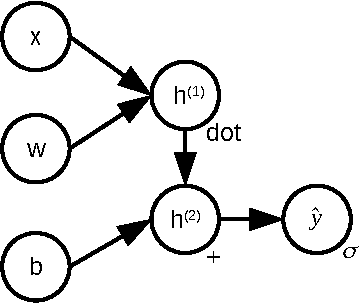
\includegraphics[width=0.4\linewidth]{./Figures/back_prop-crop.pdf}
	\caption{Computational graph with one hidden layer. The nodes in the first layer store the input $x$, weight $w$ and the bias $b$. The second layer contains the hidden layer with 2 units each with the corresponding operation written below. The final layer is the output layer denoted by  $\hat{y}=\sigma(wx+b)$, where $\sigma$ is the sigmoid function defined earlier.}
	\label{fig:graph}
\end{figure}

The gradients in the backpropagation algorithm are calculated by recursively applying the chain rule of calculus. The chain rule is a process of computing derivatives of functions based on multiple functions whose derivatives are already known. Back-propagation is an efficient implementation of chain rule with an order of operations feasible for computation. Let the input $x$,$b$ and $w$ to be real numbers, and $h^{1}$,$h^{2}$ and $\hat{y}$ be functions mapping from one real number to another, the chain rule can be written as follows:

\begin{equation}
\frac{d y}{d x}=\frac{d y}{d h^{2}} \frac{d h^{2}}{d h^{1}} \frac{d h^{1}}{d x}
\end{equation}

where $h^{1}=xw$, $h^{2}=h^{1}+b$ from Figure~\ref{fig:graph}. We can generalize the above for a vector case with $x,w,b \in \mathbb{R}^{m}$ as follows:

\begin{equation}
\frac{\partial y}{\partial x_{i}}=\sum_{j} \frac{\partial y}{\partial h^{1}_{j}} \frac{\partial h^{2}_{j}}{\partial h^{1}_{j}}\frac{\partial h^{1}_{j}}{\partial x_{j}}
\end{equation}

The chain rule involves many repeatable expressions which may need to be stored to avoid multiple re-computations for estimating gradients. Especially for complex neural networks it would lead to an exponentially high number of computations. A simplistic version of the backpropagation algorithm for a fully-connected \ac{MLP} is discussed in this section. For a supervised loss function $L(\hat{\boldsymbol{y}},\boldsymbol{y})$, where $\hat{\boldsymbol{y}}$ is the predicted output and $\boldsymbol{y}$ the target, forward propagation for a single training example is shown in Algorithm~\ref{alg:forward}. After the forward propagation the gradient on the cost function $J$ is calculated and then propagated through the network through back-propagation described in Algorithm~\ref{alg:backprop}. 
\begin{algorithm}
	\SetAlgoLined
	Number of layers, $l$ \;
    Network weights represented by matrices, $\boldsymbol{W}^{(i)},i \in \{1,\dots,l\}$ \;
	Bias parameters, $\boldsymbol{b}^{(i)},i \in \{1,\dots,l\}$ \;
	Hidden units, $h^{(i)}, i \in \{1,\dots,n\}$ \;
    
	$h^{(0)} = \boldsymbol{x} $, \Comment{Initializing input nodes} \;
    
    \For{$j =1,\dots,l$}{
		$a^{(j)}= b^{(j)} + \boldsymbol{W}^{(j)}h^{(j-1)}$ 	\Comment{information from previous layers}\; 
		$h^{(j)}= f(a^{(j)})$                               \Comment{activation in the current layer}\;
		}
	$\hat{\boldsymbol{y}} = h^{(l)}$			\;
	$J = L(\hat{\boldsymbol{y}},\boldsymbol{y}) + \lambda R(\theta)$ \Comment{Cost function with a regularization} \;
	\caption{Forward propagation algorithm for a single input example $\boldsymbol{x}$}
	\label{alg:forward}
\end{algorithm}

\begin{algorithm}
	\SetAlgoLined
	Computing gradient $g$ of the output layer\;
	$g = \nabla_{\hat{\boldsymbol{y}}} J = \nabla_{\hat{\boldsymbol{y}}} L (\hat{\boldsymbol{y}},y) $
	
	\For{$j =l,l-1\dots,1$}{
		The gradient of a particular layer's output needs to be converted into gradient before activation $f$\;
		$g = \nabla_{\boldsymbol{a}^{(j)}} J = g \circ f^{'}(a^{(j)}) $ \;
		Gradients on weights and biases \;
		$\nabla_{b^{(j)}}J = g + \lambda \nabla_{b^{(j)}} R(\theta)$ \;
		$\nabla_{\boldsymbol{W}^{(j)}}J = g h^{(j-1)} + \lambda \nabla_{\boldsymbol{W}^{(j)}} R(\theta)$ \;
		Propagating the gradients through the preceding lower lowel activations\;
		$g = \nabla_{\boldsymbol{h}}J = \boldsymbol{W}^{(j)\intercal}g$
		
	}
	\caption{Backward propagation for neural network from Algorithm~\ref{alg:forward}}
	\label{alg:backprop}
\end{algorithm}

  
\section{Optimization}
Once the gradients are calculated through backpropagation algorithm, optimization procedures like gradient descent can be use to update the network parameters ($\theta$). The two algorithms in the previous section were demonstrated for a single example. In reality neural networks are often trained in parallel on multiple examples. This set of combined examples is called a batch and optimization algorithms are implemented accordingly for training in batches. In this section we discuss two of the most used optimization algorithms \ac{SGD} and ADAM. 

\subsection{Stochastic Gradient Descent}
\ac{SGD} is an implementation of the popular gradient descent algorithm for training in batches. We obtain an estimate of the gradient by averaging the gradient over a minibatch of $m$ training examples taken from the data distribution. \ac{SGD} is depicted in Algorithm~\ref{alg:sgd}.  

\begin{algorithm}
	\SetAlgoLined
	Learning rate $\epsilon_{j}$\;
	Current parameters $\theta_{k}$\;
	\While{stopping criterion is not reached}{
		From the training set, sample $m$ minibatch of examples $\{ \boldsymbol{x}^{(1)},\dots, \boldsymbol{x}^{(m)} \}$ and corresponding targets $\{ \boldsymbol{y}^{(1)},\dots, \boldsymbol{y}^{(m)} \}$ \\
		Computing average gradient: \\
		$\hat{g} = \frac{1}{m} \nabla_{\theta_{j}} \sum_{i=1}^{m} L(f(\boldsymbol{x}^{(i)},\theta_{j}),\boldsymbol{y}^{(i)})$ \\
		Update: $\theta_{j} = \theta_{j} - \epsilon \hat{g} $ \\
		
	}
	\caption{Training update at an iteration $j$ for \acf{SGD}}
	\label{alg:sgd}
\end{algorithm}

The learning rate $\epsilon_{j}$ is gradually decreased as the training progresses, due to the noise introduced by random sampling of minibatches. 

\subsection{Adam}
Adam is another optimization algorithm which incorporates adaptive learning rate and momentum for faster convergence (\cite{kingma2014adam}). Momentum introduces velocity denoted by $v$ that indicates speed and direction for parameters to update through parameter space. It is typically set to an exponentially decaying average of the negative gradient. Adam is derived from adaptive momentum. It is depicted in Algorithm~\ref{alg:adam}.

\begin{algorithm}
	\SetAlgoLined
	Step size $\epsilon$ default usually $0.001$ \;
	Exponential decay rates $\rho_{1}$ and $\rho_{2}$, typically set to $0.9$ and $0.999$ \;
	Constant $\delta$, a very small number for stabilization, usually in the order of $10^{-8}$ \;
    Parameters $\theta$ \;
    $1^{\mathrm{st}}$ and $2^{\mathrm{nd}}$ moment variables, initialized to $s=0$, $r=0$ \;
    Time step $t=0$ \;
    
	\While{stopping criterion is not reached}{
		From the training set, sample $m$ minibatch of examples $\{ \boldsymbol{x}^{(1)},\dots, \boldsymbol{x}^{(m)} \}$ and corresponding targets $\{ \boldsymbol{y}^{(1)},\dots, \boldsymbol{y}^{(m)} \}$ \\
		Computing average gradient: \\
		$\hat{g} = \frac{1}{m} \nabla_{\theta_{j}} \sum_{i=1}^{m} L(f(\boldsymbol{x}^{(i)},\theta_{j}),\boldsymbol{y}^{(i)})$ \\
		$t = t+1$ \\
		Update first momentum estimate: $s = \rho_{1}s + (1-\rho_{1})g $ \\
		Update second momentum estimate: $r = \rho_{2}r + (1-\rho_{2})g \circ g $ \\
		Correct bias in first moment: $\hat{s}= \frac{s}{1-\rho_{1}^{t}}$ \\
		Correct bias in second moment: $\hat{r}= \frac{r}{1-\rho_{2}^{t}}$ \\
		Calculate parameter update: $\Delta \theta_{j} = -\epsilon\frac{\hat{s}}{\sqrt{\hat{r}+\delta}}$\\
		Update:  $\theta = \theta + \Delta \theta$ \\
		
	}
	\caption{Adam algorithm}
	\label{alg:adam}
\end{algorithm}

\subsection{Universal Approximation Theorem}

The wide usage of neural networks is a testimony of their ability to adapt across multiple applications. This is based on the universal approximation theorem which states that a feed-forward network with a linear output layer and at least one hidden layer with a non-linear squashing activation function (like sigmoid) can approximate any function mapping from any finite dimensional discrete space to another provided that the network has enough hidden units (\cite{hornik1990universal}). This statement needs to be taken with a pinch of salt as it does not guarantee determining the optimal parameters of the network. It merely acknowledges the existence of a network that can represent the function in question. Training the network has two major challenges. One, the optimization process involved in training the network may not be able to find the network weights suitable to represent the function due to inadequate data (under-fitting problem). Two, the training could lead to a set of parameters that do not generalize well for the test data (over-fitting). Depending on the application and the data, network design is subject to change. The best network parameters that generalize well are usually obtained empirically through careful and logical experimentation. In theory a network with a single layer is sufficient to learn the representation but it would need to be very large and therefore may fail to generalize. Hence, deeper architectures with multiple hidden layers are preferred over shallow network with infeasible number of neurons. In the next section, specialized deep neural network suitable for images called \acf{CNN} is discussed. 

\section{Convolutional Neural Network}

The neural network depicted in \ref{fig:nn} is an example of densely connected network, where all the neighboring nodes are connected with one another. As the size of data increases (say large image data), and the network becomes more complex, the number of parameters increases exponentially. To address this and also to be more suitable for image data \ac{CNN}s were formulated. \ac{CNN}s are extensively used in computer vision tasks like image classification, object detection, image segmentation (\cite{voulodimos2018deep}). The three main building blocks of a \ac{CNN} are Convolution, Activation and Pooling. Each of these layers are discussed below:

\subsection{Convolution}

Images are digitally stored in the form of 2D or 3D matrices depending on the format. A convolution kernel (also known as filter) is a matrix that operates on these images and transforms them based on the kernel values. These kernel values are also known as weights in the neural network terminology. Typically, the size of the kernel is much smaller than that of the image. Many sets of these kernels form the convolution layer of the \ac{CNN}.  The movement of the kernel over the image can be made either by a single pixel or multiple pixels. This step size is called stride ($s$). The resulting output of a convolution between filter and image is called a feature map. Consider a kernel $h$ and input image $f$ with $m$ rows and $n$ columns. Convolution between $h$ and $f$ results in a feature map $g$: 
\begin{equation}
g[m, n]=(h * f)[m, n]=\sum_{i} \sum_{j} h[i, j] f[m-i, n-j]
\end{equation}

\begin{figure}[!htbp]
	\centering
	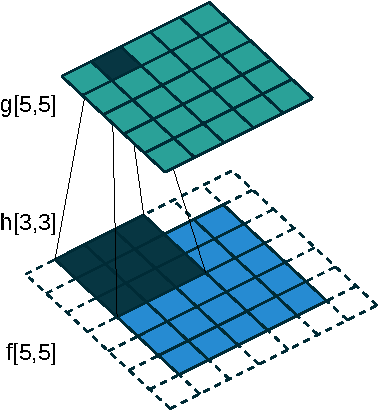
\includegraphics[width=0.4\linewidth]{./Figures/convol-crop.pdf}
	\caption{Convolution of an input image of dimensions 5$\times$5 with a filter of dimensions 3$\times$3.(\cite{dumoulin2016guide})}
	\label{fig:conv}
\end{figure}

Given in Fig~\ref{fig:conv} is a representation of the convolution operation. Zero padding is used to manipulate the dimensions of the feature maps. In the above Figure above it is indicated with dotted lines. The function of padding here is to maintain same dimensions in the input image $f$ and the feature map $g$. A \ac{CNN} learns features from the input through many convolutional layers. The earlier layers learn general features like edges, contrast, the deep layers learn more abstract and finer details.  

\subsection{Activation Layer}

The activation layer that follows the convolution layer in a \ac{CNN} is most commonly the \ac{ReLU} activation function, depicted in Fig~\ref{fig:relu}.

\begin{figure}[!htbp]
	\centering
	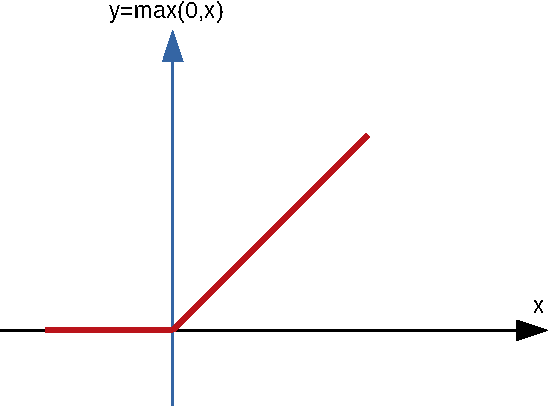
\includegraphics[width=0.6\linewidth]{relu-crop.pdf}
	\caption{The \ac{ReLU} function}
	\label{fig:relu}
\end{figure}


Many of the task based on images are non-linear in nature. Whether a computer vision task like identifying objects in an image or a medical imaging task involving tumor detection, the relationships are far from being linear. The \ac{ReLU} function increases this required non-linearity in the \ac{CNN}. 

\subsection{Pooling Layer}

The third building block of a \ac{CNN} is the pooling layer. Pooling operation is mainly used to reduce the dimensions of a tensor which enables faster computation. Max pooling is the most commonly used pooling operation. A max pooling operator of a particular size returns the maximum value of a selected region in the feature map. Similar to a filter it is implemented with a specific stride. A max pooling filter with $s=2$ is depicted in Fig~\ref{fig:mp}.

\begin{figure}[!htbp]
	\centering
	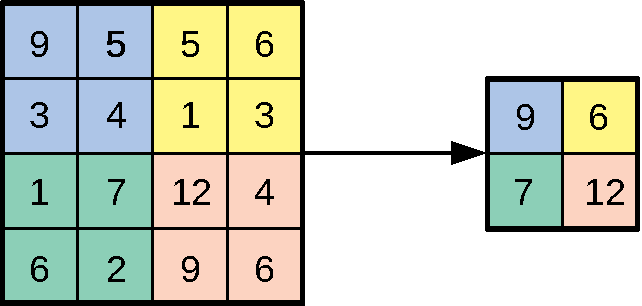
\includegraphics[width=0.6\linewidth]{maxP-crop.pdf}
	\caption{Max pooling with 2$\times$2 filter and stride 1}
	\label{fig:mp}
\end{figure}


A \ac{CNN} with $2$ convolutional layers, $2$ activation layers and $2$ pooling layers is represented in Fig~\ref{fig:trad_cnn}. Layer number is given by $l$. The first and the last layer are the input and output respectively. Usually the last set of layers in a \ac{CNN} used for classification, regression tasks is a fully-connected layer which is similar to the neural network represented in Fig~\ref{fig:nn}. With the advent of powerful computation tools and efficient parallel processing, neural networks with many layers could be implemented. The term deep learning was coined for networks with this "deep" design (\cite{lecun2015deep}). Deep neural networks could be trained over large datasets and they outperformed many existing state of the art algorithms in computer vision. In this thesis we focus specifically on \ac{CNN}s under the umbrella of deep neural networks.  




\begin{figure}[t!]
	\centering
	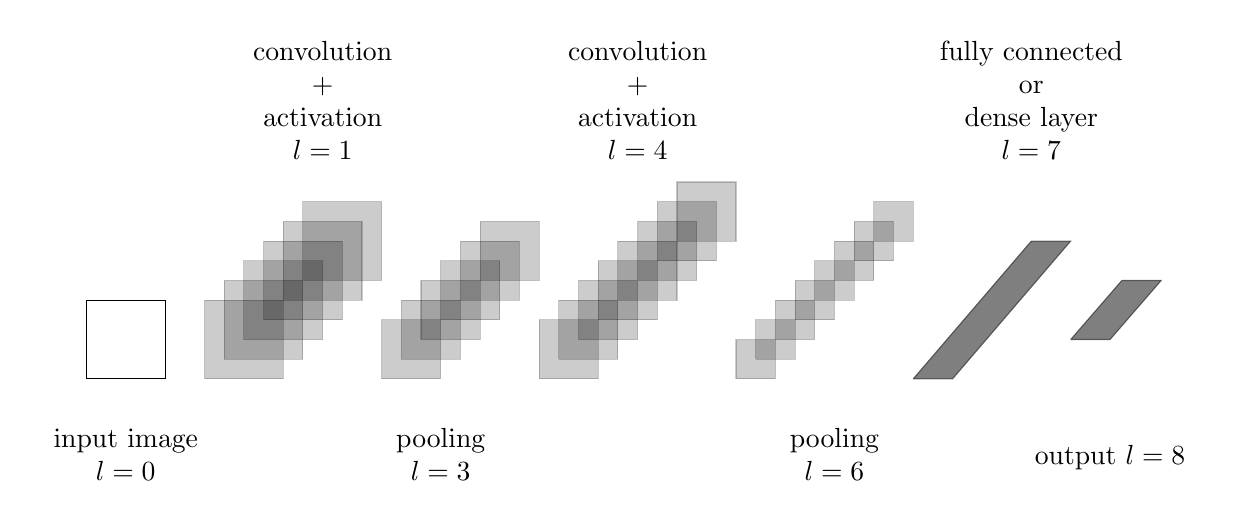
\begin{tikzpicture}
	\node at (0.5,-1){\begin{tabular}{c}input image\\ $l = 0$\end{tabular}};
	
	\draw (0,0) -- (1,0) -- (1,1) -- (0,1) -- (0,0);
	
	\node at (3,3.5){\begin{tabular}{c}convolution \\+\\ activation\\ $l = 1$\end{tabular}};
	
	\draw[fill=black,opacity=0.2,draw=black] (2.75,1.25) -- (3.75,1.25) -- (3.75,2.25) -- (2.75,2.25) -- (2.75,1.25);
	\draw[fill=black,opacity=0.2,draw=black] (2.5,1) -- (3.5,1) -- (3.5,2) -- (2.5,2) -- (2.5,1);
	\draw[fill=black,opacity=0.2,draw=black] (2.25,0.75) -- (3.25,0.75) -- (3.25,1.75) -- (2.25,1.75) -- (2.25,0.75);
	\draw[fill=black,opacity=0.2,draw=black] (2,0.5) -- (3,0.5) -- (3,1.5) -- (2,1.5) -- (2,0.5);
	\draw[fill=black,opacity=0.2,draw=black] (1.75,0.25) -- (2.75,0.25) -- (2.75,1.25) -- (1.75,1.25) -- (1.75,0.25);
	\draw[fill=black,opacity=0.2,draw=black] (1.5,0) -- (2.5,0) -- (2.5,1) -- (1.5,1) -- (1.5,0);
	
	\node at (4.5,-1){\begin{tabular}{c}pooling \\ $l = 3$\end{tabular}};
	
	\draw[fill=black,opacity=0.2,draw=black] (5,1.25) -- (5.75,1.25) -- (5.75,2) -- (5,2) -- (5,1.25);
	\draw[fill=black,opacity=0.2,draw=black] (4.75,1) -- (5.5,1) -- (5.5,1.75) -- (4.75,1.75) -- (4.75,1);
	\draw[fill=black,opacity=0.2,draw=black] (4.5,0.75) -- (5.25,0.75) -- (5.25,1.5) -- (4.5,1.5) -- (4.5,0.75);
	\draw[fill=black,opacity=0.2,draw=black] (4.25,0.5) -- (5,0.5) -- (5,1.25) -- (4.25,1.25) -- (4.25,0.5);
	\draw[fill=black,opacity=0.2,draw=black] (4,0.25) -- (4.75,0.25) -- (4.75,1) -- (4,1) -- (4,0.25);
	\draw[fill=black,opacity=0.2,draw=black] (3.75,0) -- (4.5,0) -- (4.5,0.75) -- (3.75,0.75) -- (3.75,0);
	
	\node at (7,3.5){\begin{tabular}{c}convolution \\+\\ activation\\ $l = 4$\end{tabular}};
	
	\draw[fill=black,opacity=0.2,draw=black] (7.5,1.75) -- (8.25,1.75) -- (8.25,2.5) -- (7.5,2.5) -- (7.5,1.75);
	\draw[fill=black,opacity=0.2,draw=black] (7.25,1.5) -- (8,1.5) -- (8,2.25) -- (7.25,2.25) -- (7.25,1.5);
	\draw[fill=black,opacity=0.2,draw=black] (7,1.25) -- (7.75,1.25) -- (7.75,2) -- (7,2) -- (7,1.25);
	\draw[fill=black,opacity=0.2,draw=black] (6.75,1) -- (7.5,1) -- (7.5,1.75) -- (6.75,1.75) -- (6.75,1);
	\draw[fill=black,opacity=0.2,draw=black] (6.5,0.75) -- (7.25,0.75) -- (7.25,1.5) -- (6.5,1.5) -- (6.5,0.75);
	\draw[fill=black,opacity=0.2,draw=black] (6.25,0.5) -- (7,0.5) -- (7,1.25) -- (6.25,1.25) -- (6.25,0.5);
	\draw[fill=black,opacity=0.2,draw=black] (6,0.25) -- (6.75,0.25) -- (6.75,1) -- (6,1) -- (6,0.25);
	\draw[fill=black,opacity=0.2,draw=black] (5.75,0) -- (6.5,0) -- (6.5,0.75) -- (5.75,0.75) -- (5.75,0);
	
	\node at (9.5,-1){\begin{tabular}{c}pooling\\ $l = 6$\end{tabular}};
	
	\draw[fill=black,opacity=0.2,draw=black] (10,1.75) -- (10.5,1.75) -- (10.5,2.25) -- (10,2.25) -- (10,1.75);
	\draw[fill=black,opacity=0.2,draw=black] (9.75,1.5) -- (10.25,1.5) -- (10.25,2) -- (9.75,2) -- (9.75,1.5);
	\draw[fill=black,opacity=0.2,draw=black] (9.5,1.25) -- (10,1.25) -- (10,1.75) -- (9.5,1.75) -- (9.5,1.25);
	\draw[fill=black,opacity=0.2,draw=black] (9.25,1) -- (9.75,1) -- (9.75,1.5) -- (9.25,1.5) -- (9.25,1);
	\draw[fill=black,opacity=0.2,draw=black] (9,0.75) -- (9.5,0.75) -- (9.5,1.25) -- (9,1.25) -- (9,0.75);
	\draw[fill=black,opacity=0.2,draw=black] (8.75,0.5) -- (9.25,0.5) -- (9.25,1) -- (8.75,1) -- (8.75,0.5);
	\draw[fill=black,opacity=0.2,draw=black] (8.5,0.25) -- (9,0.25) -- (9,0.75) -- (8.5,0.75) -- (8.5,0.25);
	\draw[fill=black,opacity=0.2,draw=black] (8.25,0) -- (8.75,0) -- (8.75,0.5) -- (8.25,0.5) -- (8.25,0);
	
	\node at (12,3.5){\begin{tabular}{c}fully connected\\ or\\ dense layer\\$l = 7$\end{tabular}};
	
	\draw[fill=black,draw=black,opacity=0.5] (10.5,0) -- (11,0) -- (12.5,1.75) -- (12,1.75) -- (10.5,0);
	
	\node at (13,-1){\begin{tabular}{c}output $l = 8$\end{tabular}};
	
	\draw[fill=black,draw=black,opacity=0.5] (12.5,0.5) -- (13,0.5) -- (13.65,1.25) -- (13.15,1.25) -- (12.5,0.5);
	\end{tikzpicture}
	\caption{Architecture of a typical \ac{CNN}. This representation was first proposed by \cite{lecun1995convolutional}.}
	\label{fig:trad_cnn}
\end{figure}


\subsection{Neural Networks for Image to Image Translation}

Image to image translation tasks require the \ac{CNN} to map from image in one domain to an image in another related domain. This requires the design of the \ac{CNN} to be quite different from the one depicted in Fig~\ref{fig:trad_cnn}. Convolution and pooling operations compress the input to obtain an abstract representation in lower dimensions. This lower dimensional encoding is transformed back into an image through the use of transposed convolution operators. In contrast to the compressing nature of convolutions, they expand the input feature map. The combination of convolution+pooling and transposed convolutions are adjusted depending on the dimensions of the input and output images. Transposed convolution is shown in Fig~\ref{fig:tc}. Essentially the transposed convolution spatially reverses the dimensions of the convolution+pooling operation. These networks with two parts where one part downsamples the input image and the other part upsamples the encoding into an image are called encoder-decoder networks. Since we use convolutions for achieving this encoder-decoder setup they are specifically called as \acf{CED}. 

\begin{figure}[!htbp]
	\centering
	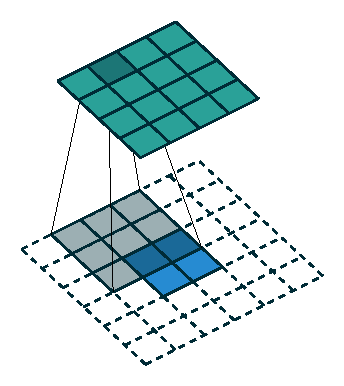
\includegraphics[width=0.4\linewidth]{transposed.pdf}
	\caption{Transposed convolution over a $2\times2$ input to get a $4\times4$ output. (\cite{dumoulin2016guide})}
	\label{fig:tc}
\end{figure}

\acp{CED} are used in a variety of image to image translation tasks. Across the literature one would find many variations used in super resolution, image segmentation, denoising and image reconstruction. This subset of \acp{CNN} appropriate for image reconstruction task is represented in Fig~\ref{fig:ced}. 

\begin{figure}[!htbp]
	\centering
	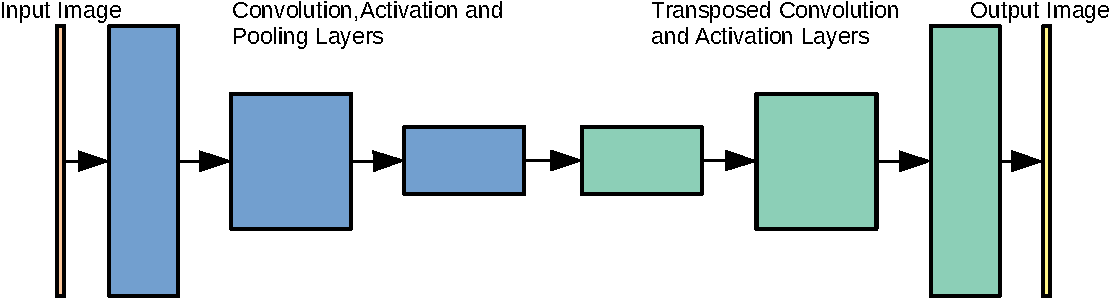
\includegraphics[width=1.0\linewidth]{fcn-crop.pdf}
	\caption{\ac{CNN} for image to image translation tasks. This example has an identical structure in convolution path and the transposed convolution path.}
	\label{fig:ced}
\end{figure}

The building blocks described in this section essentially form the basis of neural network approaches proposed in this thesis. The next chapter consists of a review of existing works in deep learning applied to medical image reconstruction. And the following chapters describe the proposed methods. 



